\documentclass[12pt,a4]{article}
\usepackage{physics, amsmath,amsfonts,amsthm,amssymb, mathtools,steinmetz, gensymb, siunitx}	% LOADS USEFUL MATH STUFF
\usepackage{xcolor,graphicx}
\usepackage[left=45pt, top=60pt, right=45pt, bottom=65pt ,a4paper]{geometry} 				% ADJUSTS PAGE
\usepackage{setspace}
\usepackage{caption}
\usepackage{adjustbox}
\usepackage{tikz}
\usepackage{pgf,tikz,pgfplots,wrapfig}
\usepackage{mathrsfs}
\usepackage{fancyhdr}
\usepackage{float}
\usepackage{array}
\usepackage{booktabs,multirow}
\usepackage{bm}
\usepackage{ulem}
\usepackage{fancyvrb}
\usepackage{rotating}


\usetikzlibrary{decorations.text, calc}
\pgfplotsset{compat=1.7}

\usetikzlibrary{decorations.pathreplacing,decorations.markings,matrix,calc}
\usepgfplotslibrary{fillbetween}

\newcommand{\vect}[1]{\boldsymbol{#1}}

\usepackage{hyperref}
%\usepackage[style= ACM-Reference-Format, maxbibnames=6, minnames=1,maxnames = 1]{biblatex}
%\addbibresource{references.bib}


\AtBeginDocument{\hypersetup{pdfborder={0 0 0}}}

\title{
\textsc{Architecture Prac 2}
}
\author{\textsc{J L Gouws}
}
\date{\today
\\[1cm]}



\usepackage{graphicx}
\usepackage{array}

\VerbatimFootnotes


\begin{document}
\thispagestyle{empty}

\maketitle

\textbf{Part 1}
\begin{enumerate}
  \item
    $\SI{2.5}{\giga\hertz}$ clock $\Rightarrow \SI{0.4}{\nano\second}$ per clock cycle.
    If the CPU executes two instructions per clock cycle, then the average time per instruction is $\SI{0.2}{\nano\second}$.
  \item
    L1 is fully-pipelined so there is no additional cost to access L1.
    Execution of instructions that do not stall the pipleline on average takes $0.5$ cycles per instruction, assuming the two issued instructions are not dependent.
    $90 \%$ of references to L2 cache are successful.
    This access to L2 stalls the pipeline for $10 \text{cycles } \times 0.01 \times 0.9 = 0.09 \text{ cycles}$.
    The remaining $10 \%$ are references to DRAM.
    I assume that the lookup to DRAM is done in parallel to L2 lookup.
    This access to DRAM stalls the pipeline for $100 \text{ cycles} \times 0.01 \times 0.1 = 0.1\text{ cycles}$.
    Totaling the penalties for DRAM and L2 cache results in $0.19 \text{ cycles}$.
    Assuming target branch instructions are always in L1, only loads and stores slow down the pipeline.
    Loads and stores make up $30 \%$ of instructions.
    Taking everything into account results in $0.2 + 0.3 \times 0.19 = 0.257$ cycles per instruction on average.
  \item
    DRAM takes 100 cycles to access. 
    Therefore, fitting a miss to DRAM into 100 cycles requires one DRAM access.
    The access must transfer all 32 bytes of the cache block.
    The bus width must, therefore, be 32 bytes.
  \item
    Execution of instructions that do not stall the pipleline on average takes $\frac{1}{2}$ cycles per instruction.
    $89 \%$ of references to L2 cache are successful.
    This access to L2 stalls the pipeline for $10 \text{cycles } \times 0.01 \times 0.89 = 0.089 \text{ cycles}$.
    The remaining $11 \%$ are references to DRAM.
    I assume that the lookup to DRAM is done in parallel to L2 lookup.
    This access to DRAM stalls the pipeline for $100 \text{ cycles} \times 0.01 \times 0.11 = 0.11 \text{ cycles}$.
    Totaling the penalties for DRAM and L2 cache results in $0.199 \text{ cycles}$.
    Only loads slow down the pipeline now.
    Loads make up $20 \%$ of instructions.
    Taking everything into account results in $0.2 + 0.2 \times 0.199 = 0.2398$ cycles per instruction on average.

\end{enumerate}

\textbf{Part 2}
\begin{enumerate}
  \item
    \begin{enumerate}
      \item
        \begin{adjustbox}{angle=-90, center}
          \begin{tabular}{l c c c c c c c c c c c c c c c c c c c c c c c}
            \textbf{instruction}& 1 & 2 & 3 & 4 & 5 & 6 & 7 & 8 & 9 & 10 & 11 & 12 & 13 & 14 & 15 & 16 & 17 & 18 & 19 & 20 & 21 & 22 & 23\\
            li  R4, 0           & F & D & X & M & W &   &   &   \\
            j   fortest         &   & F & D & X & M & W &   &   \\
            blt R4, R3, forbody &   &   & F & D & X & M & W &   \\
            lw R5, 0(R1)        &   &   &   & F & D & X & M & W \\
            lw R6, 0(R2)        &   &   &   &   & F & D & X & M & W \\
            add R5, R5, R6      &   &   &   &   &   & F & D & X & M & W \\
            sw R5, 0(R1)        &   &   &   &   &   &   & F & D & X & M & W \\
            addi R4, R4, 1      &   &   &   &   &   &   &   & F & D & X & M & W \\
            addi R1, R1, 4      &   &   &   &   &   &   &   &   & F & D & X & M & W \\
            addi R2, R2, 4      &   &   &   &   &   &   &   &   &   & F & D & X & M & W \\
            blt R4, R3, forbody &   &   &   &   &   &   &   &   &   &   & F & D & X & M & W &  \\
            lw R5, 0(R1)        &   &   &   &   &   &   &   &   &   &   &   & F & D & X & M & W \\
            lw R6, 0(R2)        &   &   &   &   &   &   &   &   &   &   &   &   & F & D & X & M & W \\
            add R5, R5, R6      &   &   &   &   &   &   &   &   &   &   &   &   &   & F & D & X & M & W \\
            sw R5, 0(R1)        &   &   &   &   &   &   &   &   &   &   &   &   &   &   & F & D & X & M & W \\
            addi R4, R4, 1      &   &   &   &   &   &   &   &   &   &   &   &   &   &   &   & F & D & X & M & W \\
            addi R1, R1, 4      &   &   &   &   &   &   &   &   &   &   &   &   &   &   &   &   & F & D & X & M & W \\
            addi R2, R2, 4      &   &   &   &   &   &   &   &   &   &   &   &   &   &   &   &   &   & F & D & X & M & W \\
            blt R4, R3, forbody &   &   &   &   &   &   &   &   &   &   &   &   &   &   &   &   &   &   & F & D & X & M & W \\
          \end{tabular}
        \end{adjustbox}
      \item
        \begin{adjustbox}{angle=-90, center, max width = 0.55\textheight}
          \begin{minipage}[t]{1.1\textheight}
            For branches, the control unit will fetch the instruction after the branch.
            The control unit fetches the branch's target instuction after it decodes the branch.\\

            \begin{tabular}{l c c c c c c c c c c c c c c c c c c c c c c c c c c c c c}
              \toprule
              \textbf{instruction}& 1 & 2 & 3 & 4 & 5 & 6 & 7 & 8 & 9 & 10 & 11 & 12 & 13 & 14 & 15 & 16 & 17 & 18 & 19 & 20 & 21 & 22 & 23 & 24 & 25 & 26 & 27 & 28 & 29\\
              \midrule
              li  R4, 0           & F & D & X & M & W &   &   &   &     \\
              \hline
              j   fortest         &   & F & D & X & M & W &   &   &     \\
              \hline
              blt R4, R3, forbody &   &   & F & D & X & M & W &   &     \\
              \hline
              \textbf{next instruction}    &   &   &   & F & \sout{D} & \sout{X} & \sout{M} & \sout{W} &   &     \\
              \hline
              lw R5, 0(R1)        &   &   &   &   & F & D & X & M & W &     \\
              \hline
              lw R6, 0(R2)        &   &   &   &   &   & F & D & X & M & W   \\
              \hline
              add R5, R5, R6      &   &   &   &   &   &   & F & D & --& X & M & W \\
              \hline
              sw R5, 0(R1)        &   &   &   &   &   &   &   & F & --& D & --& X & M & W \\
              \hline
              addi R4, R4, 1      &   &   &   &   &   &   &   &   & --& F & --& D & X & M & W \\
              \hline
              addi R1, R1, 4      &   &   &   &   &   &   &   &   & --&   & --& F & D & X & M & W \\
              \hline
              addi R2, R2, 4      &   &   &   &   &   &   &   &   & --&   & --&   & F & D & X & M & W \\
              \hline
              blt R4, R3, forbody &   &   &   &   &   &   &   &   & --&   & --&   &   & F & D & X & M & W &  \\
              \hline
              \textbf{next instruction}    &   &   &   &   &   &   &   &   &   &   &   &   &   &   & F & \sout{D} & \sout{X} & \sout{M} & \sout{W} &   &     \\
              \hline
              lw R5, 0(R1)        &   &   &   &   &   &   &   &   & --&   & --&   &   &   &   & F & D & X & M & W \\
              \hline
              lw R6, 0(R2)        &   &   &   &   &   &   &   &   & --&   & --&   &   &   &   &   & F & D & X & M & W \\
              \hline
              add R5, R5, R6      &   &   &   &   &   &   &   &   & --&   & --&   &   &   &   &   &   & F & D & --& X & M & W \\
              \hline
              sw R5, 0(R1)        &   &   &   &   &   &   &   &   & --&   & --&   &   &   &   &   &   &   & F & --& D & --& X & M & W \\
              \hline
              addi R4, R4, 1      &   &   &   &   &   &   &   &   & --&   & --&   &   &   &   &   &   &   &   & --& F & --& D & X & M & W \\
              \hline
              addi R1, R1, 4      &   &   &   &   &   &   &   &   & --&   & --&   &   &   &   &   &   &   &   & --&   & --& F & D & X & M & W \\
              \hline
              addi R2, R2, 4      &   &   &   &   &   &   &   &   & --&   & --&   &   &   &   &   &   &   &   & --&   & --&   & F & D & X & M & W \\
              \hline
              blt R4, R3, forbody &   &   &   &   &   &   &   &   & --&   & --&   &   &   &   &   &   &   &   & --&   & --&   &   & F & D & X & M & W \\
              \bottomrule
            \end{tabular}
          \end{minipage}
        \end{adjustbox}
    \end{enumerate}
  \item
    A 2-level branch predictor would not make a difference in this case.
  \item
    \begin{enumerate}
      \item
        This diagram shows the name dependences with blue arrows, and actual dependencies with red arrows.\\
        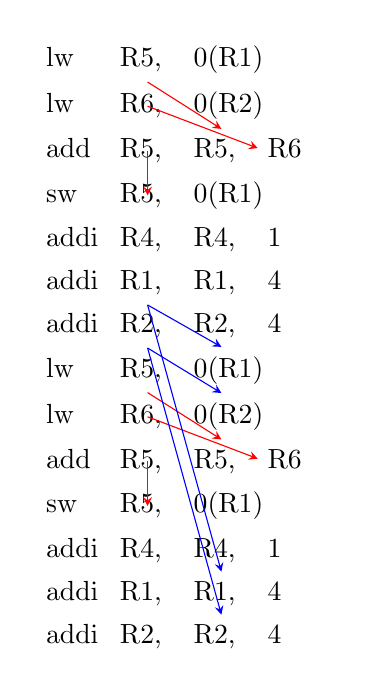
\begin{tikzpicture}[> = stealth, baseline = (current bounding box.north), text width = 2em]
          \matrix (mat) [matrix of nodes] {
              lw   & R5, & 0(R1) \\
              lw   & R6, & 0(R2) \\
              add  & R5, & R5, & R6 \\
              sw   & R5, & 0(R1) \\
              addi & R4, & R4, & 1 \\
              addi & R1, & R1, & 4 \\
              addi & R2, & R2, & 4 \\
              lw   & R5, & 0(R1) \\
              lw   & R6, & 0(R2) \\
              add  & R5, & R5, & R6 \\
              sw   & R5, & 0(R1) \\
              addi & R4, & R4, & 1 \\
              addi & R1, & R1, & 4 \\
              addi & R2, & R2, & 4 \\
          };
          \draw[->, red] (mat-1-2.south) -- (mat-3-3.north);
          \draw[->, red] (mat-2-2.center) -- (mat-3-4.west);
          \draw[->, red] (mat-3-2.center) -- (mat-4-2.center);
          \draw[->, red] (mat-8-2.south) -- (mat-10-3.north);
          \draw[->, red] (mat-9-2.center) -- (mat-10-4.west);
          \draw[->, red] (mat-10-2.center) -- (mat-11-2.center);
          \draw[->, blue] (mat-6-2.south) -- (mat-8-3.north);
          \draw[->, blue] (mat-6-2.south) -- (mat-13-3.north);
          \draw[->, blue] (mat-7-2.south) -- (mat-9-3.north);
          \draw[->, blue] (mat-7-2.south) -- (mat-14-3.north);
        \end{tikzpicture}\\

        Using very aggressive renaming and reordering, this can become.
        The renaming removes the name dependencies.

        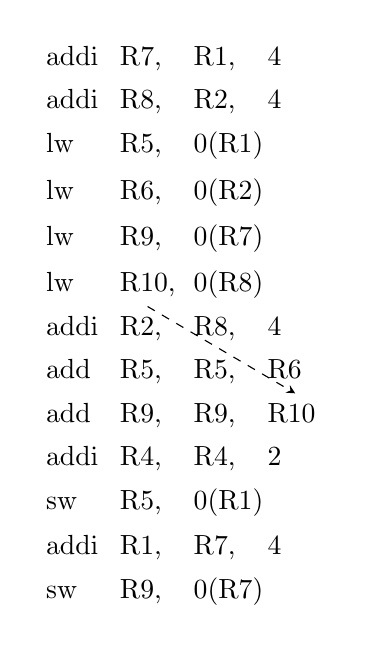
\begin{tikzpicture}[> = stealth, baseline = (current bounding box.north), text width = 2em]
          \matrix (mat) [matrix of nodes] {
              addi & R7, & R1, & 4 \\
              addi & R8, & R2, & 4 \\
              lw   & R5, & 0(R1) \\
              lw   & R6, & 0(R2) \\
              lw   & R9, & 0(R7) \\
              lw   & R10, & 0(R8) \\
              addi & R2, & R8, & 4 \\
              add  & R5, & R5, & R6 \\
              add  & R9, & R9, & R10 \\
              addi & R4, & R4, & 2 \\
              sw   & R5, & 0(R1) \\
              addi & R1, & R7, & 4 \\
              sw   & R9, & 0(R7) \\
          };
          \draw[->, dashed] (mat-6-2.south) -- (mat-9-4.north);
%          \draw[->, dashed] ($(mat-7-2.south) + (-0.3, 0) $) -- ($(mat-10-2.north) + (0.1, 0)$);
%          \draw[->, dashed] ($(mat-9-2.south) + (-0.3, 0)$) -- ($(mat-12-2.north) + (0.1, 0)$);
        \end{tikzpicture}\\
        The dashed arrow indicates the closest actual dependency. 
        The closest dependency is separated by two instructions.
      \item
        With this reordering and renaming there should not be any pipeline stalls for the loop body.
        The only stall would occur in the branch for the next loop iteration.
        It also removes one of the additions to R4, the loop counter
        The above ordering reduces all pipeline stalls.
      \item
        Tomasulo's algorithm would allow hardware to unroll the loop.
        The hardware unrolling from Tomasulo's algorithm would work for both even and odd iteration counts.
    \end{enumerate}

\end{enumerate}

\end{document}
